\documentclass[]{article}

\usepackage{amsmath}
\usepackage{amsfonts}
\usepackage{amsthm}
\usepackage{amssymb}
\usepackage{mathrsfs}
\usepackage{stmaryrd}
\usepackage{tikz}
\usetikzlibrary{calc}

\newcommand{\Q}{\mathbb{Q}}
\newcommand{\N}{\mathbb{N}}
\newcommand{\Z}{\mathbb{Z}}
\newcommand{\R}{\mathbb{R}}
\newcommand{\Primes}{\mathbb{P}}
\newcommand{\st}{\text{ s.t. }}
\newcommand{\txtand}{\text{ and }}
\newcommand{\txtor}{\text{ or }}
\newcommand{\lxor}{\veebar}

%opening
\title{Notes on Constrained Optimization}
\author{DSBA Mathematics Refresher 2026}
\date{}

\begin{document}
	
	\maketitle
	
	\begin{abstract}
		
	\end{abstract}
	
	This session will explore different methods for constrained optimization, with a particular focus on the Lagrange multiplier technique.
	
	\section{Unconstrained Optimization}
	
	Unconstrained optimization refers to the problem of optimizing a function without any restrictions or constraints on the variables.
	Mathematically, this can be expressed as:
	$$
	\text{Find } \mathbf{x}^* \text{ such that } f(\mathbf{x}^*) = \min_{\mathbf{x}} f(\mathbf{x})
	$$
	where $f(\mathbf{x})$ is the objective function.
	
	The necessary condition for \(\mathbf{x}^*\) to be an extremum is that the gradient of $f$ at $\mathbf{x}^*$ is zero:
	$$
	\nabla f(\mathbf{x}^*) = \mathbf{0}
	$$
	
	\subsection{Direct Calculation Method}
	The direct method involves taking the derivative of the function with respect to each variable, setting these derivatives equal to zero, and solving the resulting system of equations.
	
	\textbf{Example:}
	\noindent\\
	Consider the function $f(x, y) = x^2 + y^2$. To find the minimum, we calculate:
	$$
	\frac{\partial f}{\partial x} = 2x, \quad \frac{\partial f}{\partial y} = 2y
	$$
	Setting these equal to zero, we get:
	$$
	2x = 0 \quad \text{and} \quad 2y = 0
	$$
	This gives $x = 0$ and $y = 0$, which is the minimum point.
	
	\subsection{Iterative Process}
	In a previous session, we explored iterative process to find the extremum of a function.
	This is often used when solving $\nabla f(\mathbf{x}^*) = \mathbf{0}$ can not be done in reasonable time.
	
	\section{Constrained Optimization}
	In many practical problems, the optimization process is subject to certain constraints.
	These constraints can be either equality or inequality constraints.
	
	\subsection{Equality Constrained Optimization}
	Equality constrained optimization problems can be expressed as:
	$$
	\text{Minimize } f(\mathbf{x})
	\quad
	\text{subject to}
	\quad
	g_i(\mathbf{x}) = 0
	\quad
	\text{for } i = 1, \dots, m
	$$
	
	\subsubsection{Direct Calculation Method}
	For some simple problems, we can solve the constraint explicitly and substitute it back into the objective function to reduce the problem to an unconstrained optimization problem.
	
	\textbf{Example:}
	Minimize $f(x, y) = x^2 + y^2$ subject to the constraint $x + y = 1$.
	\\
	Solve the constraint for $y = 1 - x$, and substitute into $f(x, y)$:
	$$
	f(x, 1-x) = x^2 + (1-x)^2 = 2x^2 - 2x + 1
	$$
	Minimize the resulting function by finding the derivative and setting it to zero:
	$$
	\frac{d}{dx}(2x^2 - 2x + 1) = 4x - 2 = 0
	$$
	This gives $x = \frac{1}{2}$, and hence $y = \frac{1}{2}$.
	
	\subsubsection{Lagrange Multiplier Method}
	The Lagrange multiplier method introduces an auxiliary variable (the Lagrange multiplier) to incorporate the constraints into the objective function.
	
	\textbf{Lagrange Function:}
	$$
	\mathcal{L}(\mathbf{x}, \lambda) = f(\mathbf{x}) - \sum_{i=1}^m \lambda_i g_i(\mathbf{x})
	$$
	To find the stationary points, we solve the system
	$$
	\nabla \mathcal{L}(\mathbf{x}, \lambda) = \mathbf{0}
	$$
	where the gradient is taken with respect to \textit{all} the variables: the $\mathbf{x}$ \textbf{and} the multipliers $\lambda_i$.

	\textit{On the sign:} some textbooks write $f + \sum \lambda_i g_i$ instead.
	This changes nothing except the sign of the $\lambda_i$, since $\lambda_i$ is unknown anyway.
	We use the minus sign throughout this course because it is the convention that makes the sign condition of the inequality case (Section 2.2) come out as $\lambda \geq 0$.

	\subsubsection{Why Does It Work?}

	The method looks like a trick pulled out of a hat: we add a term that is \textit{zero anyway} on the constraint (since $g_i(\mathbf{x}) = 0$ there), and suddenly the constrained problem becomes an unconstrained one.
	Here is where it comes from.

	\paragraph{Step 1: a gradient is perpendicular to its level sets.}
	Let $\mathbf{x}(t)$ be a path that stays inside the constraint set, so that
	$$
	g(\mathbf{x}(t)) = 0 \qquad \text{for every } t
	$$
	Differentiating this identity with respect to $t$ (chain rule):
	$$
	\nabla g(\mathbf{x}(t)) \cdot \mathbf{x}'(t) = 0
	$$
	So $\nabla g$ is perpendicular to every direction in which we may travel while respecting the constraint.
	In other words, $\nabla g$ is perpendicular to the constraint curve (or surface).

	\begin{center}
		\begin{minipage}[t]{0.46\textwidth}
			\centering
			\vspace{0pt}
			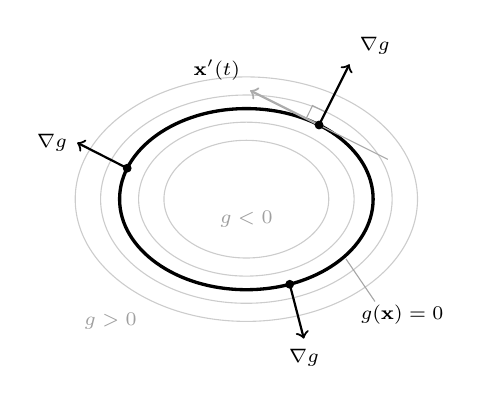
\begin{tikzpicture}[scale=1.15]
				% level curves of g; the constraint is the one where g = 0
				\draw[gray!40] (0,0) ellipse (0.91 and 0.65);
				\draw[gray!40] (0,0) ellipse (1.19 and 0.85);
				\draw[very thick] (0,0) ellipse (1.4 and 1.0);
				\draw[gray!40] (0,0) ellipse (1.61 and 1.15);
				\draw[gray!40] (0,0) ellipse (1.89 and 1.35);
				\node[gray!75] at (0,-0.22) {\scriptsize $g<0$};
				\node[gray!75] at (-1.5,-1.35) {\scriptsize $g>0$};
				\node at (1.72,-1.28) {\scriptsize $g(\mathbf{x})=0$};
				\draw[gray!70] (1.42,-1.13) -- (1.1,-0.66);
				% the point, its tangent line and the gradient there
				\draw[gray!65] (0.043,1.199) -- (1.563,0.439);
				\draw[->,gray!65,thick] (0.803,0.819) -- (0.043,1.199) node[above left,black] {\scriptsize $\mathbf{x}'(t)$};
				\draw[gray!70] (0.660,0.890) -- (0.731,1.033) -- (0.874,0.962);
				\draw[->,thick] (0.803,0.819) -- (1.138,1.490) node[above right] {\scriptsize $\nabla g$};
				\filldraw (0.803,0.819) circle (1.2pt);
				% the gradient at two other points of the constraint
				\draw[->,thick] (-1.316,0.342) -- (-1.868,0.623) node[left] {\scriptsize $\nabla g$};
				\filldraw (-1.316,0.342) circle (1.2pt);
				\draw[->,thick] (0.479,-0.940) -- (0.635,-1.540) node[below] {\scriptsize $\nabla g$};
				\filldraw (0.479,-0.940) circle (1.2pt);
			\end{tikzpicture}
			\\[0.4em]
			{\scriptsize A curve in the plane: at each of its points, $\nabla g$ is perpendicular to the curve, i.e. to the single direction $\mathbf{x}'(t)$ in which we may travel.}
		\end{minipage}
		\hfill
		\begin{minipage}[t]{0.46\textwidth}
			\centering
			\vspace{0pt}
			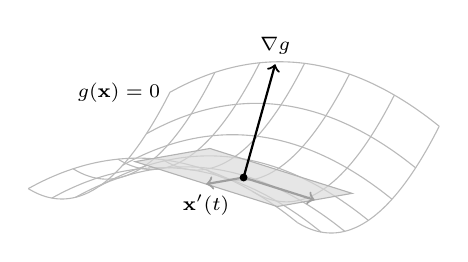
\begin{tikzpicture}[x={(-0.50cm,-0.34cm)},y={(0.95cm,-0.12cm)},z={(0cm,1.0cm)}]
				% the constraint surface g = 0, drawn as a mesh
				\foreach \v in {-1.8,-1.2,-0.6,0,0.6,1.2,1.8}
					\draw[gray!55,smooth,variable=\u,domain=-1.8:1.8]
						plot (\u,\v,{0.18*(\u*\u-\v*\v)});
				\foreach \u in {-1.8,-1.2,-0.6,0,0.6,1.2,1.8}
					\draw[gray!55,smooth,variable=\v,domain=-1.8:1.8]
						plot (\u,\v,{0.18*(\u*\u-\v*\v)});
				\node[left] at (-1.8,-1.8,0) {\scriptsize $g(\mathbf{x})=0$};
				% the tangent plane at the point: all the allowed directions at once
				\fill[gray!30,opacity=0.65] (1.65,1.45,0.1116) -- (1.65,-0.45,0.4536)
					-- (-0.25,-0.45,-0.0252) -- (-0.25,1.45,-0.3672) -- cycle;
				\draw[gray!60] (1.65,1.45,0.1116) -- (1.65,-0.45,0.4536)
					-- (-0.25,-0.45,-0.0252) -- (-0.25,1.45,-0.3672) -- cycle;
				% two allowed directions of travel, spanning that plane
				\draw[->,gray!75,thick] (0.7,0.5,0.0432) -- (1.65,0.5,0.2826) node[below,black] {\scriptsize $\mathbf{x}'(t)$};
				\draw[->,gray!75,thick] (0.7,0.5,0.0432) -- (0.7,1.45,-0.1278);
				% the gradient, perpendicular to the whole plane
				\draw[->,thick] (0.7,0.5,0.0432) -- (0.359,0.743,1.395) node[above] {\scriptsize $\nabla g$};
				\filldraw (0.7,0.5,0.0432) circle (1.2pt);
			\end{tikzpicture}
			\\[0.4em]
			{\scriptsize A surface in space: the allowed directions now fill a whole plane (the tangent plane), and $\nabla g$ is perpendicular to all of them at once.}
		\end{minipage}
	\end{center}

	\paragraph{Step 2: at a constrained optimum, $f$ does not change along the constraint.}
	Suppose $\mathbf{x}^*$ minimizes $f$ among the points satisfying the constraint, and let $\mathbf{x}(t)$ be any path inside the constraint set with $\mathbf{x}(0) = \mathbf{x}^*$.
	The function of one variable
	$$
	t \longmapsto f(\mathbf{x}(t))
	$$
	then has a minimum at $t = 0$, so its derivative vanishes there:
	$$
	\nabla f(\mathbf{x}^*) \cdot \mathbf{x}'(0) = 0
	$$
	So $\nabla f$ is \textit{also} perpendicular to every allowed direction of travel.

	\begin{center}
		\begin{minipage}[t]{0.46\textwidth}
			\centering
			\vspace{0pt}
			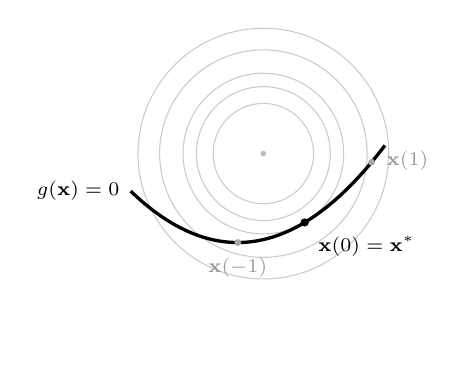
\begin{tikzpicture}[scale=0.85]
				\path (-3.1,-2.05) (2.9,2.6); % window shared by all the panels of Step 2
				% level curves of f
				\draw[gray!40] (0.383,0.729) circle (0.75);
				\draw[gray!40] (0.383,0.729) circle (1.0);
				\draw[gray!40] (0.383,0.729) circle (1.2);
				\draw[gray!40] (0.383,0.729) circle (1.55);
				\draw[gray!40] (0.383,0.729) circle (1.873);
				\filldraw[gray!55] (0.383,0.729) circle (0.9pt);
				% the constraint
				\draw[very thick,smooth,variable=\x,domain=-1.6:2.2] plot (\x,{0.3*\x*\x-0.6});
				\node[left] at (-1.62,0.168) {\scriptsize $g(\mathbf{x})=0$};
				% three positions along the path x(t)
				\filldraw[gray!70] (0,-0.6) circle (1.2pt);
				\node[gray!80,below] at (0,-0.68) {\scriptsize $\mathbf{x}(-1)$};
				\filldraw (1,-0.3) circle (1.5pt);
				\node[below right] at (1.06,-0.36) {\scriptsize $\mathbf{x}(0)=\mathbf{x}^*$};
				\filldraw[gray!70] (2,0.6) circle (1.2pt);
				\node[gray!80,right] at (2.08,0.62) {\scriptsize $\mathbf{x}(1)$};
			\end{tikzpicture}
			\\[0.4em]
			{\scriptsize Walking along the constraint through $\mathbf{x}^*$.}
		\end{minipage}
		\hfill
		\begin{minipage}[t]{0.46\textwidth}
			\centering
			\vspace{0pt}
			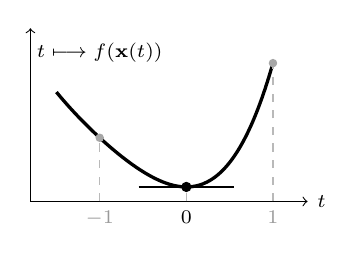
\begin{tikzpicture}[scale=1.1]
				\draw[->] (-1.8,0) -- (1.4,0) node[right] {\scriptsize $t$};
				\draw[->] (-1.8,0) -- (-1.8,2.0);
				% the one-variable function t -> f(x(t))
				\draw[very thick,smooth,variable=\t,domain=-1.5:1.0,samples=60]
					plot (\t,{1.2*((\t+0.617)*(\t+0.617)+(0.3*(1+\t)*(1+\t)-1.329)*(0.3*(1+\t)*(1+\t)-1.329)-1.3)});
				\node at (-1.0,1.72) {\scriptsize $t \longmapsto f(\mathbf{x}(t))$};
				% the two other sampled instants
				\draw[gray!55,dashed] (-1,0) -- (-1,0.735);
				\filldraw[gray!70] (-1,0.735) circle (1.2pt);
				\node[gray!80,below] at (-1,0) {\scriptsize $-1$};
				\draw[gray!55,dashed] (1,0) -- (1,1.597);
				\filldraw[gray!70] (1,1.597) circle (1.2pt);
				\node[gray!80,below] at (1,0) {\scriptsize $1$};
				% the minimum, with its horizontal tangent
				\draw[gray!55,dashed] (0,0) -- (0,0.1675);
				\draw[thick] (-0.55,0.1675) -- (0.55,0.1675);
				\filldraw (0,0.1675) circle (1.5pt);
				\node[below] at (0,0) {\scriptsize $0$};
			\end{tikzpicture}
			\\[0.4em]
			{\scriptsize The values of $f$ along that walk: a minimum at $t=0$, so the derivative vanishes and the tangent there is horizontal.}
		\end{minipage}
	\end{center}

	This is the heart of the matter, and it is worth restating in words: if $\nabla f$ had \textit{any} component along the constraint, we could slide a little in that direction, stay allowed, and decrease $f$, so we would not be at the optimum.

	\paragraph{Step 3: two vectors perpendicular to the same directions are parallel.}
	With a single constraint, the allowed directions of travel form a space of dimension $n-1$ (the tangent to the constraint surface).
	Both $\nabla f$ and $\nabla g$ are perpendicular to all of it, and the space of vectors perpendicular to a space of dimension $n-1$ has dimension $1$.
	Hence $\nabla f$ and $\nabla g$ are parallel: there exists a number $\lambda$ such that
	$$
	\boxed{\ \nabla f(\mathbf{x}^*) = \lambda \, \nabla g(\mathbf{x}^*)\ }
	$$
	This, together with the constraint $g(\mathbf{x}^*) = 0$ itself, is the real content of the method.
	The number $\lambda$ appears simply as the proportionality factor between two parallel vectors.

	\begin{center}
		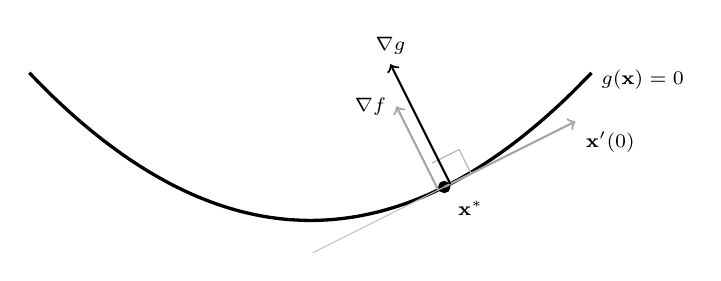
\begin{tikzpicture}[scale=1.7]
			% the constraint curve g = 0
			\draw[very thick,domain=-2.1:2.1,smooth,variable=\x] plot (\x,{0.25*\x*\x});
			\node[right] at (2.1,1.05) {\scriptsize $g(\mathbf{x})=0$};
			% the point x*
			\filldraw (1,0.25) circle (1.2pt);
			\node[below right] at (1.03,0.22) {\scriptsize $\mathbf{x}^*$};
			% tangent direction (allowed direction of travel)
			\draw[gray!50] (1,0.25) -- ++(-0.98,-0.49);
			\draw[->,gray!70,thick] (1,0.25) -- ++(0.98,0.49) node[below right,black] {\scriptsize $\mathbf{x}'(0)$};
			% right angle mark
			\draw[gray!60] ($(1,0.25)+(0.20,0.10)$) -- ++(-0.089,0.179) -- ++(-0.20,-0.10);
			% the two parallel gradients
			\draw[->,thick] ($(1,0.25)+(0.045,0.023)$) -- ++(-0.447,0.894) node[above] {\scriptsize $\nabla g$};
			\draw[->,thick,gray!70] ($(1,0.25)-(0.045,0.023)$) -- ++(-0.313,0.626) node[left,black] {\scriptsize $\nabla f$};
		\end{tikzpicture}
	\end{center}
	Both gradients are perpendicular to the \textit{same} line of allowed travel, so they must point along the same axis: they are parallel.

	\paragraph{Step 4: the Lagrangian is just bookkeeping.}
	We now have two conditions to satisfy simultaneously:
	$$
	\nabla f = \lambda \nabla g
	\qquad \text{and} \qquad
	g(\mathbf{x}) = 0
	$$
	Look at what the Lagrangian does with them.
	Differentiating $\mathcal{L} = f - \lambda g$ with respect to the $\mathbf{x}$ variables gives
	$$
	\nabla_\mathbf{x} \mathcal{L} = \nabla f - \lambda \nabla g = \mathbf{0}
	\qquad \Longleftrightarrow \qquad
	\nabla f = \lambda \nabla g
	$$
	which is the first condition; and differentiating with respect to $\lambda$ gives
	$$
	\frac{\partial \mathcal{L}}{\partial \lambda} = -g(\mathbf{x}) = 0
	\qquad \Longleftrightarrow \qquad
	g(\mathbf{x}) = 0
	$$
	which is the second one (the constraint comes back by itself).

	So the Lagrangian is not magic: it is a device that packs the geometric condition \textit{and} the constraint into a single equation $\nabla \mathcal{L} = \mathbf{0}$, which we can then hand to the usual unconstrained machinery.
	Treating $\lambda$ as one more variable is exactly what makes the constraint reappear.

	\paragraph{The same picture with level curves.}
	Imagine walking along the constraint curve while watching the level curves of $f$.
	As long as you are crossing level curves, $f$ is changing, so you can keep going down.
	You stop descending exactly when the constraint curve stops crossing the level curves and \textit{touches} one instead, that is, when the two curves are \textbf{tangent}.
	Two curves are tangent exactly when their normals are parallel, i.e. when $\nabla f = \lambda \nabla g$.

	\noindent \textbf{Example:}
	For $f(x,y) = x^2+y^2$ with the constraint $g(x,y) = x + y - 1 = 0$:
	$$
	\nabla f = \begin{pmatrix} 2x \\ 2y \end{pmatrix}
	\qquad \text{and} \qquad
	\nabla g = \begin{pmatrix} 1 \\ 1 \end{pmatrix}
	$$
	These are parallel exactly when $2x = 2y$, i.e. $x = y$; combined with the constraint, this gives $x = y = \frac{1}{2}$ straight away.
	The level curves of $f$ are circles centred on the origin, and the answer is the point where the line $x+y=1$ is tangent to one of them (the closest point of the line to the origin, as expected).

	\begin{center}
		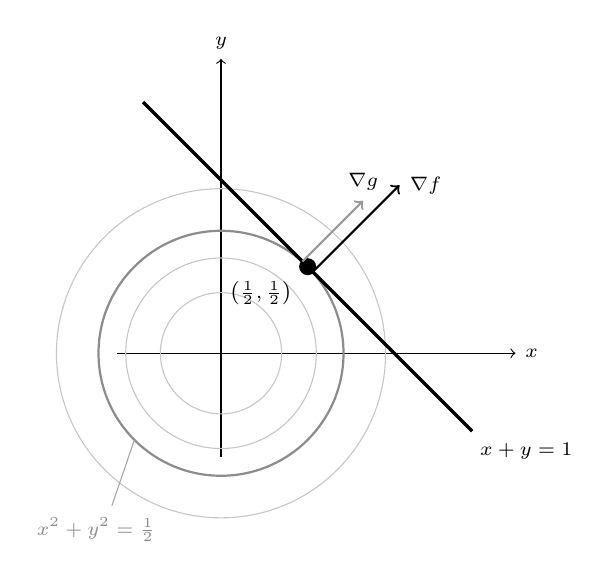
\begin{tikzpicture}[scale=2.2]
			\draw[->] (-0.6,0) -- (1.7,0) node[right] {\scriptsize $x$};
			\draw[->] (0,-0.6) -- (0,1.7) node[above] {\scriptsize $y$};
			% level curves of f: circles centred at the origin
			\draw[gray!45] (0,0) circle (0.35);
			\draw[gray!45] (0,0) circle (0.55);
			\draw[thick,gray!90] (0,0) circle (0.7071);
			\draw[gray!45] (0,0) circle (0.95);
			\node[gray!90] at (-0.72,-1.02) {\scriptsize $x^2+y^2=\frac{1}{2}$};
			\draw[gray!70] (-0.63,-0.88) -- (-0.5,-0.5);
			% the constraint line x + y = 1
			\draw[very thick] (-0.45,1.45) -- (1.45,-0.45);
			\node[below right] at (1.44,-0.46) {\scriptsize $x+y=1$};
			% the tangency point
			\filldraw (0.5,0.5) circle (1.3pt);
			\node[below left] at (0.47,0.47) {\scriptsize $\left(\frac{1}{2},\frac{1}{2}\right)$};
			% the two parallel gradients
			\draw[->,thick] (0.53,0.47) -- ++(0.5,0.5) node[right] {\scriptsize $\nabla f$};
			\draw[->,thick,gray!80] (0.47,0.53) -- ++(0.35,0.35) node[above,black] {\scriptsize $\nabla g$};
		\end{tikzpicture}
	\end{center}
	Walking along the line from either side, we cross smaller and smaller circles; we stop descending exactly where the line \textit{touches} one instead of crossing it.
	There, the normal to the line ($\nabla g$) and the normal to the level curve ($\nabla f$) point in the same direction, and the multiplier $\lambda$ is the ratio of their lengths.

	\paragraph{Warnings:}
	\begin{itemize}
		\item \textbf{Do not try to minimize $\mathcal{L}$.}
		The solution is a \textit{stationary} point of $\mathcal{L}$, not a minimum of it: $\mathcal{L}$ typically has a saddle point there (it is minimal in $\mathbf{x}$, but maximal in $\lambda$).
		Only $\nabla \mathcal{L} = \mathbf{0}$ matters.
		\item \textbf{The argument needs $\nabla g \neq \mathbf{0}$.}
		If $\nabla g$ vanishes at the solution, Step 3 collapses (the "direction perpendicular to the constraint" is not well defined) and the method can miss the answer.
		This is rare in practice, but it is the reason the theorem always comes with such an assumption.
	\end{itemize}

	\paragraph{With several constraints.}
	The same reasoning applies: the allowed directions are those perpendicular to \textit{all} the $\nabla g_i$ at once, and $\nabla f$ must again be perpendicular to all of them.
	This forces $\nabla f$ to be a linear combination of the $\nabla g_i$:
	$$
	\nabla f = \sum_{i=1}^m \lambda_i \nabla g_i
	$$
	which is precisely $\nabla_\mathbf{x} \mathcal{L} = \mathbf{0}$ for the Lagrangian written above, with one multiplier per constraint.

	\textbf{Example:}
	Minimize $f(x, y) = x^2 + y^2$ subject to $x + y = 1$.

	\textbf{Step 1: Construct the Lagrange Function}\\
	The Lagrangian is:
	$$
	\mathcal{L}(x, y, \lambda) = x^2 + y^2 - \lambda (x + y - 1)
	$$

	\textbf{Step 2: Compute the Partial Derivatives}\\
	The partial derivatives of the Lagrangian are:
	$$
	\frac{\partial \mathcal{L}}{\partial x} = 2x - \lambda = 0, \quad \frac{\partial \mathcal{L}}{\partial y} = 2y - \lambda = 0, \quad \frac{\partial \mathcal{L}}{\partial \lambda} = -(x + y - 1) = 0
	$$
	Note how the last one simply hands the constraint back to us.

	\textbf{Step 3: Solve the System of Equations}\\
	The first two equations give $x = y = \frac{\lambda}{2}$; substituting into the third (i.e. into the constraint) gives $\lambda = 1$, hence $x = y = \frac{1}{2}$, which matches our previous result.
	
	\textbf{Step 4: Determine the Optimal Point}\\
	Substitute $x = \frac{1}{2}$, $y = \frac{1}{2}$ into the original function:
	$$
	f\left(\frac{1}{2}, \frac{1}{2}\right) = \left(\frac{1}{2}\right)^2 + \left(\frac{1}{2}\right)^2 = \frac{1}{4} + \frac{1}{4} = \frac{1}{2}
	$$
	Thus, the minimum value of $f(x, y) = x^2 + y^2$ subject to $x + y = 1$ is $\frac{1}{2}$ at the point $\left(\frac{1}{2}, \frac{1}{2}\right)$.

	\textbf{Example:}
	A Less Friendly Constraint\\
	Find the extreme values of $f(x, y) = x + y$ on the ellipse
	$$
	\frac{x^2}{4} + y^2 = 1
	$$
	Here the substitution method is already painful: solving the constraint gives $y = \pm\sqrt{1 - \frac{x^2}{4}}$, that is two branches, each carrying a square root that we would then have to differentiate and discuss separately.
	The Lagrangian does not care.

	\textbf{Step 1: Construct the Lagrange Function}\\
	With $g(x, y) = \frac{x^2}{4} + y^2 - 1$, the Lagrangian is:
	$$
	\mathcal{L}(x, y, \lambda) = x + y - \lambda \left( \frac{x^2}{4} + y^2 - 1 \right)
	$$

	\textbf{Step 2: Compute the Partial Derivatives}\\
	$$
	\frac{\partial \mathcal{L}}{\partial x} = 1 - \lambda \frac{x}{2} = 0,
	\quad
	\frac{\partial \mathcal{L}}{\partial y} = 1 - 2 \lambda y = 0,
	\quad
	\frac{\partial \mathcal{L}}{\partial \lambda} = -\left( \frac{x^2}{4} + y^2 - 1 \right) = 0
	$$

	\textbf{Step 3: Solve the System of Equations}\\
	The first two equations force $\lambda \neq 0$ (with $\lambda = 0$ they would read $1 = 0$), so we may divide by it:
	$$
	x = \frac{2}{\lambda}
	\qquad \text{and} \qquad
	y = \frac{1}{2\lambda}
	$$
	Note that this is the whole point of the method: instead of eliminating $y$ against a square root, we have expressed \textit{both} unknowns in terms of the single multiplier.
	Substituting them into the third equation (the constraint) leaves one equation in $\lambda$ alone:
	$$
	\frac{1}{4} \cdot \frac{4}{\lambda^2} + \frac{1}{4 \lambda^2} = 1
	\qquad \Longleftrightarrow \qquad
	\frac{5}{4 \lambda^2} = 1
	\qquad \Longleftrightarrow \qquad
	\lambda = \pm \frac{\sqrt{5}}{2}
	$$

	\textbf{Step 4: Determine the Optimal Points}\\
	Each sign gives one stationary point:
	$$
	\lambda = \frac{\sqrt{5}}{2}
	\ \longrightarrow \
	\left( \frac{4}{\sqrt{5}}, \frac{1}{\sqrt{5}} \right),
	\qquad
	\lambda = -\frac{\sqrt{5}}{2}
	\ \longrightarrow \
	\left( -\frac{4}{\sqrt{5}}, -\frac{1}{\sqrt{5}} \right)
	$$
	Both satisfy the constraint, as $\frac{16/5}{4} + \frac{1}{5} = \frac{4}{5} + \frac{1}{5} = 1$.
	The method stops here: it has produced two candidates without saying which is which, so we compare the values of $f$:
	$$
	f\left( \frac{4}{\sqrt{5}}, \frac{1}{\sqrt{5}} \right) = \frac{5}{\sqrt{5}} = \sqrt{5},
	\qquad
	f\left( -\frac{4}{\sqrt{5}}, -\frac{1}{\sqrt{5}} \right) = -\sqrt{5}
	$$
	So the maximum of $f$ on the ellipse is $\sqrt{5}$ and the minimum is $-\sqrt{5}$.

	Geometrically, the level curves of $f$ are the lines $x + y = c$.
	Sliding such a line across the plane, the extreme values of $c$ are those for which the line still touches the ellipse, and the two tangency points are exactly the two solutions found above.
	
	\subsection{Inequality Constrained Optimization}
	Inequality constrained optimization problems can be expressed as:
	$$
	\text{Minimize } f(\mathbf{x})
	\quad
	\text{subject to}
	\quad
	g_i(\mathbf{x}) \geq 0
	\quad
	\text{for } i = 1, \dots, m
	$$
	
	\subsubsection{Direct Method}
	When the constraint is active (i.e., it holds as an equality), it can be treated similarly to the equality-constrained case.
	If inactive, it is ignored.
	
	\textbf{Example:}
	Minimizing a Quadratic Function with an Inequality Constraint
	\\
	Minimize $f(x, y) = x^2 + y^2$ subject to $x \geq 0$ and $y \geq 0$.
	\\
	This can be approached by checking the boundary and interior points.
	The minimum will be at $(0,0)$ given the non-negative constraints.
	\\
	Note that if the constraint was $x+y \geq 1$, showing that the minimum is at $(0.5, 0.5)$ is much harder via direct calculations.
	
	\subsubsection{Lagrange Multiplier Method with Slack Variables}
	We note that:
	$$
	g_i(\mathbf{x}) \geq 0
	\iff
	g_i(\mathbf{x}) -s^2 = 0
	\quad
	\text{ for some } s \in \R
	$$
	Here, $s$ is called a "slack variable".
	It is then possible to use the Lagrange trick as before.
	\\
	The Lagrange multiplier method introduces now multiple auxiliary variables: the Lagrange multiplier and some slack variables to incorporate the inequality constraints into the objective function.
	
	\textbf{Lagrange Function:}
	$$
	\mathcal{L}(\mathbf{x}, \mathbf{s}, \lambda)
	= f(\mathbf{x}) - \sum_{i=1}^m \lambda_i \left( g_i(\mathbf{x}) - s_i^2 \right)
	$$
	To find the stationary points, we solve the system
	$$
	\nabla \mathcal{L}(\mathbf{x}, \mathbf{s}, \lambda) = \mathbf{0}
	\qquad \text{together with} \qquad
	\lambda_i \geq 0
	$$
	where, again, the gradient is taken with respect to every variable: the $\mathbf{x}$, the slack variables $s_i$, and the multipliers $\lambda_i$.

	\subsubsection{Why Does It Work?}

	Everything of the equality case still applies (after all, we have turned the inequalities into equalities).
	Two new things happen, and both are worth understanding.

	\paragraph{The derivative in $s$ produces a case distinction.}
	Differentiating $\mathcal{L}$ with respect to a slack variable $s_i$ gives
	$$
	\frac{\partial \mathcal{L}}{\partial s_i} = 2 \lambda_i s_i = 0
	$$
	A product is zero when one of its factors is, so \textit{for each constraint}:
	$$
	\lambda_i = 0
	\qquad \text{or} \qquad
	s_i = 0
	$$
	These two cases are exactly the two things that can happen to an inequality constraint:
	\begin{itemize}
		\item $s_i = 0$ means $g_i(\mathbf{x}) = s_i^2 = 0$: the constraint holds \textit{as an equality}, we are on its boundary.
		The constraint is \textbf{active}, and we are back to the equality case.
		\item $\lambda_i = 0$ means the constraint term disappears from $\mathcal{L}$ altogether: the optimum is the same as if the constraint had never been written.
		The constraint is \textbf{inactive}.
	\end{itemize}
	This is why solving these problems always splits into cases, and it is the whole reason for introducing $s$: the slack variable is what \textit{detects} whether a constraint is doing any work.
	The property
	$$
	\lambda_i \, g_i(\mathbf{x}) = 0 \qquad \text{for every } i
	$$
	(one of the two factors is always zero) is known as \textbf{complementary slackness}.

	\paragraph{The multiplier must have the right sign.}
	This is the one genuinely new condition, and the reason it exists is that an inequality, unlike an equality, has a \textit{direction}.

	Suppose the constraint $g(\mathbf{x}) \geq 0$ is active at the solution, so we sit on the boundary $g = 0$, and recall from the equality case that $\nabla f = \lambda \nabla g$ there.
	Now, $\nabla g$ points towards increasing $g$, that is, \textit{towards the inside} of the allowed region.
	We are at a genuine minimum only if $f$ increases as we step inside (otherwise we would step in and do better).
	The increase of $f$ in the direction $\nabla g$ is
	$$
	\nabla f \cdot \nabla g = \lambda \, \nabla g \cdot \nabla g = \lambda \, \|\nabla g\|^2
	$$
	and since $\|\nabla g\|^2 > 0$, this is positive exactly when
	$$
	\lambda \geq 0
	$$
	So the sign condition is not a technicality: it is what distinguishes "the constraint is holding the solution back" (genuine constrained minimum, $\lambda > 0$) from "the constraint is pushing the solution outwards" (not a minimum at all, $\lambda < 0$).
	A negative multiplier is how the method tells us that we have found the wrong kind of point, and that the case should be discarded.

	\begin{center}
		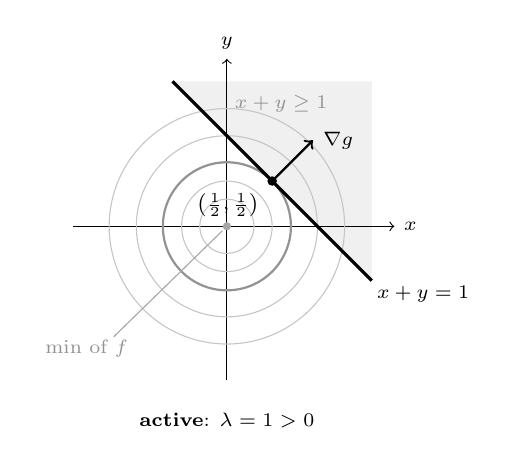
\begin{tikzpicture}[scale=1.15]
			\path (-2.2,-2.35) (2.1,1.95); % common bounding box, so both pictures align
			% feasible region x + y >= 1
			\fill[gray!12] (-0.6,1.6) -- (1.6,-0.6) -- (1.6,1.6) -- cycle;
			\draw[->] (-1.7,0) -- (1.85,0) node[right] {\scriptsize $x$};
			\draw[->] (0,-1.7) -- (0,1.85) node[above] {\scriptsize $y$};
			% level curves of f
			\draw[gray!45] (0,0) circle (0.3);
			\draw[gray!45] (0,0) circle (0.5);
			\draw[thick,gray!85] (0,0) circle (0.7071);
			\draw[gray!45] (0,0) circle (1.0);
			\draw[gray!45] (0,0) circle (1.3);
			% the constraint
			\draw[very thick] (-0.6,1.6) -- (1.6,-0.6);
			\node[below right] at (1.55,-0.55) {\scriptsize $x+y=1$};
			\node[gray!85] at (0.6,1.35) {\scriptsize $x+y\geq1$};
			% unconstrained minimum, now forbidden
			\filldraw[gray!70] (0,0) circle (1.1pt);
			\node[gray!85] at (-1.55,-1.35) {\scriptsize min of $f$};
			\draw[gray!70] (-1.25,-1.22) -- (-0.05,-0.05);
			% the constrained optimum
			\filldraw (0.5,0.5) circle (1.3pt);
			\node[below left] at (0.47,0.47) {\scriptsize $\left(\frac{1}{2},\frac{1}{2}\right)$};
			\draw[->,thick] (0.5,0.5) -- ++(0.45,0.45) node[right] {\scriptsize $\nabla g$};
			\node at (0,-2.15) {\scriptsize \textbf{active}: $\lambda = 1 > 0$};
		\end{tikzpicture}
		\hspace{0.5cm}
		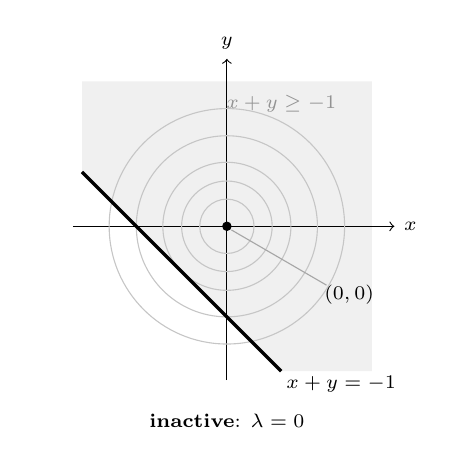
\begin{tikzpicture}[scale=1.15]
			\path (-2.2,-2.35) (2.1,1.95); % same window as the picture on the left
			% feasible region x + y >= -1
			\fill[gray!12] (-1.6,0.6) -- (0.6,-1.6) -- (1.6,-1.6) -- (1.6,1.6) -- (-1.6,1.6) -- cycle;
			\draw[->] (-1.7,0) -- (1.85,0) node[right] {\scriptsize $x$};
			\draw[->] (0,-1.7) -- (0,1.85) node[above] {\scriptsize $y$};
			% level curves of f
			\draw[gray!45] (0,0) circle (0.3);
			\draw[gray!45] (0,0) circle (0.5);
			\draw[gray!45] (0,0) circle (0.7071);
			\draw[gray!45] (0,0) circle (1.0);
			\draw[gray!45] (0,0) circle (1.3);
			% the constraint, never reached
			\draw[very thick] (-1.6,0.6) -- (0.6,-1.6);
			\node[below right] at (0.55,-1.55) {\scriptsize $x+y=-1$};
			\node[gray!85] at (0.6,1.35) {\scriptsize $x+y\geq-1$};
			% the optimum: the unconstrained one
			\filldraw (0,0) circle (1.3pt);
			\node at (1.35,-0.75) {\scriptsize $(0,0)$};
			\draw[gray!70] (1.1,-0.65) -- (0.05,-0.04);
			\node at (0,-2.15) {\scriptsize \textbf{inactive}: $\lambda = 0$};
		\end{tikzpicture}
	\end{center}
	On the left the unconstrained minimum $(0,0)$ is forbidden: the solution is pushed onto the boundary, the constraint is active and $\lambda > 0$.
	On the right the same unconstrained minimum already satisfies the constraint: the boundary is never reached, the constraint is inactive and $\lambda = 0$.
	Notice how, in the active case, $\nabla g$ points \textit{into} the allowed region, and so must $\nabla f = \lambda \nabla g$, which is precisely the statement $\lambda \geq 0$.

	Note also that this is where our sign convention pays off: had we written $\mathcal{L} = f + \lambda(g - s^2)$, the very same reasoning would give $\lambda \leq 0$ instead.

	\paragraph{Summary of the conditions.}
	Putting everything together, at a solution there are numbers $\lambda_i$ such that
	$$
	\nabla f = \sum_{i=1}^m \lambda_i \nabla g_i,
	\qquad
	g_i(\mathbf{x}) \geq 0,
	\qquad
	\lambda_i \geq 0,
	\qquad
	\lambda_i \, g_i(\mathbf{x}) = 0
	$$
	These are the \textbf{Karush-Kuhn-Tucker (KKT) conditions}, and they are the foundation of most of constrained optimization, including the Support Vector Machines of the Binary Classification session.

	\textbf{Example:}
	Minimizing a Quadratic Function with an Inequality Constraint\\
	Consider the problem of minimizing the function $f(x, y) = x^2 + y^2$ subject to the inequality constraint $x + y \geq 1$.
	
	\textbf{Step 1: Introduce the Slack Variable}\\
	The constraint can be written as:
	$$
	x + y - s^2 = 1 \quad \text{as } s^2 \geq 0 \quad \forall s \in \mathbb{R}
	$$
	where $s$ is the slack variable.
	The constraint is now an equality constraint.
	
	\textbf{Step 2: Construct the Lagrange Function}\\
	The Lagrange function incorporating the constraint is:
	$$
	\mathcal{L}(x, y, s, \lambda) = x^2 + y^2 - \lambda \left( (x + y) - s^2 - 1 \right)
	$$
	where $\lambda$ is the Lagrange multiplier.
	
	\textbf{Step 3: Compute the Partial Derivatives}\\
	To find the stationary points, take the partial derivatives of $\mathcal{L}$ with respect to $x$, $y$, $s$, and $\lambda$, and set them to zero:
	$$
	\frac{\partial \mathcal{L}}{\partial x} = 2x - \lambda = 0
	$$
	$$
	\frac{\partial \mathcal{L}}{\partial y} = 2y - \lambda = 0
	$$
	$$
	\frac{\partial \mathcal{L}}{\partial s} = 2\lambda s = 0
	$$
	$$
	\frac{\partial \mathcal{L}}{\partial \lambda} = -\left( x + y - s^2 - 1 \right) = 0
	$$
	
	\textbf{Step 4: Solve the System of Equations}\\
	From $\frac{\partial \mathcal{L}}{\partial x} = 0$ and $\frac{\partial \mathcal{L}}{\partial y} = 0$, we have:
	$$
	2x - \lambda = 0 \quad \text{and} \quad 2y - \lambda = 0
	$$
	This implies $x = y$.\\
	From $\frac{\partial \mathcal{L}}{\partial s} = 0$, we have:
	$$
	2\lambda s = 0
	$$
	This implies $\lambda = 0$ or $s = 0$. 
	
	\begin{enumerate}
		\item If $\lambda = 0$, then $x = 0$ and $y = 0$, but this would violate the constraint $x + y \geq 1$.
		Hence, this case is not valid.
		\item If $s = 0$, the constraint simplifies to $x + y = 1$.
		Since $x = y$, we have $2x = 1$, so $x = \frac{1}{2}$ and $y = \frac{1}{2}$.
		The multiplier is then $\lambda = 2x = 1 \geq 0$, as required: the constraint is active, and it is genuinely holding the solution back.
	\end{enumerate}
	
	\textbf{Step 5: Determine the Optimal Point}\\
	Substitute $x = \frac{1}{2}$, $y = \frac{1}{2}$ into the original function:
	$f\left(\frac{1}{2}, \frac{1}{2}\right) = \frac{1}{2}$.
	Thus, the minimum value of $f(x, y) = x^2 + y^2$ subject to $x + y \geq 1$ is $\frac{1}{2}$ at the point $\left(\frac{1}{2}, \frac{1}{2}\right)$.

	\textbf{Example:}
	Two Inequality Constraints\\
	Minimize
	$$
	f(x, y) = (x-3)^2 + (y-2)^2
	\qquad \text{subject to} \qquad
	x + y \leq 4
	\quad \text{and} \quad
	x \geq 0
	$$
	In words: find the allowed point closest to the target $(3,2)$.
	This time there are two constraints, so there are two multipliers and two slack variables, and the case analysis becomes the real work.

	\textbf{Step 1: Write the Constraints in the Standard Form}\\
	Our convention is $g_i \geq 0$, so we set:
	$$
	g_1(x, y) = 4 - x - y \geq 0
	\qquad \text{and} \qquad
	g_2(x, y) = x \geq 0
	$$

	\textbf{Step 2: Construct the Lagrange Function}\\
	With one slack variable per constraint:
	$$
	\mathcal{L}(x, y, s_1, s_2, \lambda_1, \lambda_2)
	= (x-3)^2 + (y-2)^2
	- \lambda_1 \left( 4 - x - y - s_1^2 \right)
	- \lambda_2 \left( x - s_2^2 \right)
	$$

	\textbf{Step 3: Compute the Partial Derivatives}\\
	$$
	\frac{\partial \mathcal{L}}{\partial x} = 2(x-3) + \lambda_1 - \lambda_2 = 0,
	\qquad
	\frac{\partial \mathcal{L}}{\partial y} = 2(y-2) + \lambda_1 = 0
	$$
	$$
	\frac{\partial \mathcal{L}}{\partial s_1} = 2 \lambda_1 s_1 = 0,
	\qquad
	\frac{\partial \mathcal{L}}{\partial s_2} = 2 \lambda_2 s_2 = 0
	$$
	$$
	\frac{\partial \mathcal{L}}{\partial \lambda_1} = -\left( 4 - x - y - s_1^2 \right) = 0,
	\qquad
	\frac{\partial \mathcal{L}}{\partial \lambda_2} = -\left( x - s_2^2 \right) = 0
	$$

	\textbf{Step 4: Solve the System of Equations}\\
	Each of the two products $\lambda_i s_i = 0$ offers two possibilities, which leaves $2 \times 2 = 4$ cases to examine.
	Remember that $s_i = 0$ means "constraint $i$ active" and $\lambda_i = 0$ means "constraint $i$ inactive".

	\begin{enumerate}
		\item $\lambda_1 = 0$ and $\lambda_2 = 0$ (no constraint doing any work).
		The first two equations become $2(x-3) = 0$ and $2(y-2) = 0$, giving the unconstrained minimum $(3,2)$.
		But then $g_1 = 4 - 3 - 2 = -1 < 0$: the point is not allowed.
		The slack variable says the same thing, as $s_1^2 = 4 - x - y = -1$ has no real solution.
		This case is rejected.

		\item $s_1 = 0$ and $\lambda_2 = 0$ (only $x + y \leq 4$ active).
		Subtracting the second equation from the first (with $\lambda_2 = 0$) eliminates $\lambda_1$:
		$$
		2(x-3) = 2(y-2)
		\qquad \Longleftrightarrow \qquad
		x = y + 1
		$$
		Together with $s_1 = 0$, that is $x + y = 4$, this gives $y = \frac{3}{2}$ and $x = \frac{5}{2}$.
		The multipliers are $\lambda_1 = -2(y-2) = 1 \geq 0$ and $\lambda_2 = 0$, and the second constraint holds, as $x = \frac{5}{2} \geq 0$.
		Everything checks out, so this candidate is kept.

		\item $\lambda_1 = 0$ and $s_2 = 0$ (only $x \geq 0$ active).
		Here $x = 0$ and the second equation gives $y = 2$, a point which is indeed allowed ($g_1 = 2 \geq 0$).
		The first equation, however, gives:
		$$
		2(0-3) - \lambda_2 = 0
		\qquad \Longleftrightarrow \qquad
		\lambda_2 = -6 < 0
		$$
		The sign condition fails, so this case is rejected.
		Geometrically, the constraint $x \geq 0$ is pushing the point outwards rather than holding it back: from $(0,2)$ we can move to the right, stay allowed, and get closer to $(3,2)$.

		\item $s_1 = 0$ and $s_2 = 0$ (both constraints active).
		Then $x = 0$ and $x + y = 4$, so the point is the corner $(0,4)$.
		The second equation gives:
		$$
		2(4-2) + \lambda_1 = 0
		\qquad \Longleftrightarrow \qquad
		\lambda_1 = -4 < 0
		$$
		The sign condition fails again, and the case is rejected.
	\end{enumerate}

	\textbf{Step 5: Determine the Optimal Point}\\
	Only one case survived, so the minimum is:
	$$
	f\left( \frac{5}{2}, \frac{3}{2} \right)
	= \left( -\frac{1}{2} \right)^2 + \left( -\frac{1}{2} \right)^2
	= \frac{1}{2}
	$$
	Thus, the closest allowed point to $(3,2)$ is $\left( \frac{5}{2}, \frac{3}{2} \right)$, at squared distance $\frac{1}{2}$.

	Note what the two multipliers tell us.
	The first one, $\lambda_1 = 1 > 0$, says that $x + y \leq 4$ is active and genuinely holding the solution back (relaxing it would improve $f$).
	The second one, $\lambda_2 = 0$, says that $x \geq 0$ is inactive: the optimum would be exactly the same if we had never written that constraint.
	This is complementary slackness at work, and it is what makes the case analysis worth the trouble: the method finds \textit{by itself} which constraints matter.
	
\end{document}
